\chapter{First Order Ordinary Differential Equations (\ode{}s)}
\section{Introduction}
As mentioned in the previous chapter, the order is determined by the highest derivative appearing in the equation.
For a first order differential equation, only $y'$ appears.

A first-order ordinary differential equation is an equation involving an unknown function $y(x)$ and its first derivative $y'(x)$. The general form is:
\[
y' = f(x,y).
\]

We will explore several common types of first-order ODEs and the methods used to solve them.

\bigskip

First-order differential equations can be classified into several types:

\begin{table}[htbp]
    \centering
    \label{tab:ode_summary}
    \begin{tabular}{>{\bfseries}l >{$}l<{$} p{8cm}}
        \toprule
        \textbf{Type} & \textbf{General Form} & \textbf{Method} \\
        \midrule
        Separable & \frac{dy}{dx} = g(x)h(y) & Rewrite as $\frac{dy}{h(y)} = g(x)\,dx$ and integrate both sides. \\
        \addlinespace
        Linear & y' + P(x)y = Q(x) & Use an integrating factor $\mu(x) = e^{\int P(x)\,dx}$. Multiply the equation by $\mu(x)$, then integrate. \\
         \addlinespace
        Exact & M(x,y)\,dx + N(x,y)\,dy = 0 & Check if $\frac{\partial M}{\partial y} = \frac{\partial N}{\partial x}$. If so, find a potential function $\Phi(x,y)$ such that $d\Phi = M\,dx + N\,dy$. The solution is $\Phi(x,y)=C$. \\
        \addlinespace
        \multicolumn{3}{l}{\textbf{Special Forms}} \\
        \cmidrule{1-3}
        Bernoulli & y' + P(x)y = Q(x)y^n & Substitute $u=y^{1-n}$ to convert it to a linear equation. \\
        \addlinespace
        Homogeneous & y' = f(y/x) & Substitute $v=y/x$ to convert it to a separable equation. \\
        \bottomrule
    \end{tabular}
\end{table}


\section{Existence and Uniqueness}
Before we proceed, we need to establish the conditions under which a different equation will have a solution.
\begin{theorem}[Existence and Uniqueness for 1st Order Nonlinear Equations (Picard–Lindelöf)]
    Suppose $f(x,y)$ and $\frac{\partial f}{\partial y}$ are continuous in a rectangle $R: \alpha < x < \beta, \delta < x < \gamma $ containing \((x_0,y_0)\). Then the initial value problem
    \[
    y' = f(x,y), \quad y(x_0)=y_0
    \]
    has a unique solution in some interval around $x_0$.
\end{theorem}

\begin{theorem}[Existence and Uniqueness for 1st Order Linear Equations]
    If the functions \(P\) and \(Q\) are continuous on an open interval \(I:\alpha < x < \beta\) containing the point \(x=x_0\), then there exists a unique function \(y=\phi(x)\) that satisfies the differential equation
    \begin{equation}
        y' + P(x)y = Q(x)
    \end{equation}
    for each \(x\in I\), and that also satisfies the initial condition \(y(x_0) = y_0\).
\end{theorem}



\section{Separable Equations}
A first-order differential equation is \textbf{separable} if it can be written in the form:
$$ \frac{dy}{dx} = g(x)h(y) $$
where $g(x)$ is a function of $x$ alone and $h(y)$ is a function of $y$ alone.

\textbf{Solution Method}
\begin{enumerate}
    \item Separate the variables by rearranging the equation:
    $$ \frac{1}{h(y)} \, dy = g(x) \, dx $$
    \item Integrate both sides of the equation:
    $$ \int \frac{1}{h(y)} \, dy = \int g(x) \, dx + C $$
    \item Solve the resulting algebraic expression for $y$ to get the general solution.
\end{enumerate}

\begin{example}
Solve:
\[
    y' = xy.
    \]
    \textbf{Solution:}  
    \[
    \frac{dy}{dx} = xy \quad \Rightarrow \quad \frac{dy}{y} = x\,dx.
    \]
    Integrate:
    \[
    \ln|y| = \tfrac{1}{2}x^2 + C \quad \Rightarrow \quad y(x) = Ce^{x^2/2}.
    \]
\end{example}

\begin{example} Solve \(y' = \dfrac{x^2}{y^2}\).

    \textbf{Solution:}
    \[
    y^2 \, dy = x^2 \, dx \quad \Rightarrow \quad \int y^2 \, dy = \int x^2 \, dx
    \].
    
    Integrate both sides
    \[
    \frac{y^3}{3} = \frac{x^3}{3} + C \quad \Rightarrow \quad y^3 = x^3 + 3C
    \] 
    
    Since $3C$ is an arbitrary constant, we can write $y^3 = x^3 + K$.
    $$ y = \sqrt[3]{x^3 + K} $$

\end{example}


\begin{highlight}
    We should note that this solution method for certain kinds of differential
    equations may lead to an Integral-defined function (i.e the integral cannot 
    be written in terms of any elementary function).
\end{highlight}


\subsection*{Practice Problems}
\begin{question}
  Solve the following separable \ode{}s:
  \begin{multicols}{3}
  \begin{enumerate}[a)]
    \item $\displaystyle (2y)\, e^{y^2}y' = 1$
    \item $\displaystyle y' =\frac{\cos(3x)}{\sin^2(3x)}$
    \item $\displaystyle y' = \frac{1}{1+x^2}$
    \item $\displaystyle y' = \frac{2x}{x^2+4}$
    \item $\displaystyle y' = \frac{1}{\sqrt{1-x^2}}$
    \item $\displaystyle y' = \frac{e^{-y}}{y}$
    \item $\displaystyle y' = \frac{1}{y^2 \ln(y)}$
    \item $\displaystyle y' = e^x \cos(x)$
    \item $\displaystyle y' = -\ln(y)$
    \item $\displaystyle y' = \frac{1}{x^2-1}$.
    \item $\displaystyle y' = \frac{3x+5}{(x+1)(x-2)}$.
    \item $\displaystyle y' = \frac{2x}{x^2+3x+2}$.
    \item $\displaystyle y' = \frac{x^2+1}{x(x^2+1)}$.
    \item $\displaystyle y' = \frac{1}{(x+1)^2(x-2)}$.
\end{enumerate}
\end{multicols}
\end{question}

\begin{question}
  Solve the following separable \ode{}
  \begin{enumerate}[a)]
  \item $\displaystyle y' = x e^{x^2}$.
  \item $\displaystyle y' = \frac{\ln(x)}{x^2}$.
  \item $\displaystyle y' = \sqrt{4-y^2}$.
  \item $\displaystyle y' = \frac{\arctan(x)}{1+x^2}$.
\end{enumerate}
\end{question}

\begin{question}
  Solve the following separable \ode{}s:
  \begin{multicols}{3}
  \begin{enumerate}[a)]
    \item $\displaystyle y' = y^2 \sin(x)$
    \item $\displaystyle y' = y^3 x$
    \item $\displaystyle y' = (y^2-1)x$
    \item $\displaystyle y' = (y+2)(y-1)$
    \item $\displaystyle y' = (y-1)(y-3)x^2$
    \item $\displaystyle y' = (y+1)(y-2)x e^x$
    \item $\displaystyle y' = (y^2-4)xe^{x^2}$
    \item $\displaystyle y' = (y^2-9)\cos(x)$
    \item $\displaystyle y' = (y-1)(y+3)\sin(x)$
    \item $\displaystyle y' = (y+4)(y-2)x^3$
    \item $\displaystyle y' = (y-5)(y+1)e^{-x}$
    \item $\displaystyle y' = (y^2-16)x^4$
  \end{enumerate}
  \end{multicols}
\end{question}

\begin{question}Identify the separable \ode{}s out of those given below. Demonstrate that it can be written in the standard form\index{standard form!separable} \(y'(x) = F(x) G(y)\):
  \begin{colenumerate}
  \item $y'+xy-x=0$
  \item $y'-3(y^2-5y-6) = 0$
  \end{colenumerate}
\end{question}

\begin{question}
    Solve \(\dfrac{dy}{dx} = y^2 - 4\).
\end{question}


\begin{question}
  Find the implicit formula \(F(x,y) = \text{const.}\) for the \textbf{solution} of the following separable \ode{}:
  \[
    y'(x) = (y^{2} -6y + 8) x e^{x}
  \]
\end{question}


\begin{question}
    Find the solution to the separable \ode{} \(y'(x) = y(3-y)\).
\end{question}

\begin{question}
Consider a population of bacteria that grows at a rate proportional\index{proportional} to the size of the population.
\begin{enumerate}[(a)]
\item Determine a \ode{} to describe the growth of
  bacteria at any time $t$.
\item Sketch the direction field, and make a prediction of what the solution is based on the sketch.
\item Determine the solution analytically.
\item The number of bacteria in a colony at 10:00am is approximately five million. At
noon the number is approximately seven million. How many bacteria were in the colony at
9:00am?
\end{enumerate}
\end{question}

\begin{question}Determine the equilibrium solutions for each \ode{} and decide if they are
stable (an attractor), unstable (a repellor) or semistable\footnote{Do some research if you need to.}.\index{stability!stable} \index{stability!unstable} \index{stability!semistable} Draw a 1-D phase portrait for each.
  \begin{colenumerate}
  \item  $y'=(y-2)(y+1)(y+2)$
  \item $y'=y^3-9y$
  \item $y'=y^3+2y^2+y$
  \item $y'=-y-y^3$
  \end{colenumerate}
\end{question}

\begin{question}
A model for the population $P(t)$ in a suburb of a large city is given by the Initial Value Problem (IVP)\index{IVP}\footnote{IVPs are \ode{}s with additional condition that the solution or its derivatives has to take certain values at a specific point.}
\[
\frac{dP}{dt} = P(10^{-1} - 10^{-7}P), \qquad P(0) = 5000,
\]
where $t$ is measured in months. What is the limiting value\index{limit} of the population\footnote{Hint: recall equilibrium solutions}? At what time will the population be equal to one-half of this limiting value?
\end{question}

\begin{question}
Solve these IVPs:
  \begin{colenumerate}
  \item $e^x\frac{dy}{dx} = xy^2$, $y(0)=2$
  \item $\frac{dy}{dx} = y^2 +1$, $y(0) = 3$
\end{colenumerate}
\end{question}

\begin{question}
 Find the 1-parameter family of solutions for each \ode{}:
  \begin{colenumerate}
  \item $xy'+2y=e^{-x}$
  \item $x\dfrac{dy}{dx}=2y+x^4\sin(x^2)$
  \item $\dfrac{dy}{dx}+xy = xy^3$
  \item $(1+x^2)y' + 4xy = \dfrac{4x}{(1+x^2)^3}$
  \end{colenumerate}
\end{question}


\begin{question}
    Solve \(y' = e^{-x^2}, \quad y(3)=5.\)
\end{question}
\noindent See how to solve here\footnote{\url{https://math.stackexchange.com/questions/154968/is-there-really-no-way-to-integrate-e-x2}}




\section{Linear Equations}
Linear\footnote{The name comes from the \textbf{linear combination}, which is a more-general expression that appears in various parts of mathematics.} ODEs are those that can be written in the form
\[
\underbrace{a_{0}(x)y(x) + a_{1}(x)\frac{dy}{dx} + a_{2}(x)\frac{d^{2}y}{dx^{2}} + \dots a_{n}(x)\frac{d^{n}y}{dx^n}}_{\text{\textbf{Linear combination} of derivatives}} = g(x)
\]
are called \textbf{linear} ODEs. Notice: the \textbf{only way} the \textbf{dependent} variable appears in the equation is in expressions of the sort\footnote{\(y^{(k)}\) denotes the \(k\)-th derivative. So \(y^{(2)}(x) = y''(x)\).}
\[
  \dots + a_{k}(x) y^{(k)}(x) + \dots,
\]
that is \(y\) or its derivatives are never squared, multiplied with each other, or appear in more complicated formulas. The \textbf{coefficient functions} \(a_{k}(x)\) may be very complicated themselves, but they never involve \(y\) or its derivatives.\footnote{For more on linear equations, see the beginning of Zill \(\S 2.3\).}

The \textbf{standard form} of a linear ODE is obtained by dividing through by the highest coefficient, to result in expression that has a constant (\(=1\)) as its highest coefficient:
\[
\underbrace{P_{0}(x)y(x) + P_{1}(x)\frac{dy}{dx} + P_{2}(x)\frac{d^{2}y}{dx^{2}} + \dots + \mathbf{1 \cdot \frac{d^{n}y}{dx^n}}}_{\text{\textbf{Linear combination} of derivatives}} = \underbrace{Q(x)}_{\text{\textbf{Input} or \textbf{Inhomogeneity}}}.
\]
The \textbf{standard form} is the starting point for many solution algorithms.

The standard\footnote{\textbf{If you want to show that an ODE is linear}, rearrange the terms to match the standard form. If you can find such functions \(P(x)\) and \(f(x)\) that \textbf{do not depend on \(y\), \(y'\)} then you are looking at a linear ODE.}
 form for \textbf{1st order linear ODEs} is:
\[
  P(x) y(x) + y'(x) = Q(x)
\]
where $P(x)$ and $Q(x)$ are continuous functions of $x$.

Here are several examples of 1st order linear ODEs. Rearrange them into a standard form and identify their coefficient function \(P(x)\) and input function \(Q(x)\) for each of them.
  \begin{colenumerate}[2]
  \item \(y'(x) = -0.5 y(x) + 8\)
  \item \(4y'(x) = -2 y(x) + 32 + 4 \sin(x)\)
  \item \(x^{2} y'(x) + 0.5 y(x) = x^{3}\)
  \item \(y'(x) = 3 y(x)\)
  \end{colenumerate}

\begin{question}
    Which of the following differential equations are linear?
    \begin{colenumerate}[3]
        \item \(y' + 2xy = 0\)
        \item \(y' = y + 5\)
        \item \(y' + y = x\)
    \end{colenumerate}
    \noindent Is any of them separable?
\end{question}

\subsection{Solution Method using Variation of parameters}

To solve 1st order linear ODEs, we will use the \textbf{variation of parameters} method: \footnote{Textbook explains the \textbf{integrating factor} technique instead. The two methods are different, but yield equivalent results. Through variation of parameters we will learn skills that will transfer over to higher-order ODEs.}

  \begin{enumerate}[\bfseries Step (1)]
  \item Convert a linear ODE into its standard form \(y' + P(x) y = Q(x)\).
  \item Create the homogeneous subproblem by zeroing out the input function:
      \[y_{H}' + P(x) y_{H} = \textbf{0}\]
    \item Find the general solution of the homogeneous subproblem.\footnote{For 1st order ODEs, this is always possible by separation of variables.}
    \item To form \textbf{a candidate solution \(y_{I}\)} for the inhomogeneous problem 
    \begin{equation}
    y_{I}' + P(x) y_{I} = Q(x),
    \end{equation}
    replace the integration parameter \(C\) in \(y_{H}\) by an unknown function \(I(x)\). \footnote{Variation of constant \(C\) \(\to\) function \(I(x)\) is what gives the method its name.}
    \item \textbf{Substitute the candidate}\footnote{Anytime something is called ``solution candidate'' your instinct should be to ``plug it into'' the ODE.} \(y_{I}\) into the \textbf{full (original)} ODE. You will need to take its derivative first, which will contain the unknown functions \(I(x)\) and \(I'(x)\). Simplify until you get an expression \(I'(x) = \dots\).

 \(I(x)\) will not appear on the right hand side (and neither will \(y\)).
    \item Integrate \(I'(x)\) to calculate \(I(x)\) function\footnote{The integration constant inside \(I(x)\) is not important, so pick a constant that makes \(I(x)\) simple. Say \(0\).}, which then gives you formula for \(y_{I}(x)\).
    \item Now you have two functions: \(y_{H}\) and \(y_{I}\). \(y_{H}\) contains a constant \(C\), while \(y_{I}\) has no free constant. The general solution to the original problem is:
      \[
        y(x) = y_{H}(x) + y_{I}(x)
      \]
    \end{enumerate}

    \begin{example}
        Find general solution to \[xy' - 4y = x^{6}e^{x}\] (this is the same problem as textbook \S 2.3.Ex.3). Additionally, find the particular solution that has \(y(2) = 0\).

        \textbf{General solution:}

        \begin{enumerate}[\bfseries Step (1)]
          \item Standard form:
          \(
            y' +\underbrace{\dfrac{-4}{x}}_{P(x)} y = \underbrace{x^{5}e^{x}}_{f(x)}
          \)
          
          \item Homogeneous subproblem:
            \begin{equation}
              y_{H}' +\dfrac{-4}{x} y_{H} = 0
            \end{equation}
            
          \item Solving for \(y_{H}\):
            \begin{align*}
              \dfrac{dy_{H}}{dx} &= \dfrac{4 y_{H}}{x} \quad \text{\scriptsize (Separate variables)}\\
              \dfrac{dy_{H}}{y_{H}} &= \frac{4 dx}{x} \\
              \int \dfrac{dy_{H}}{y_{H}} &= \int \frac{4 dx}{x} \\
              \ln \abs{y_{H}} &= 4 \ln\abs{x} + K \quad \text{\scriptsize(Exponentiate both sides)} \\
              y_{H}(x) &= C x^{4}
            \end{align*}
          \item \textbf{Candidate solution} for the inhomogeneous problem:
            \(
              y_{I}(x) = I(x) x^{4}
            \)
          \item Substitute \(y_{I} = I(x) x^{4}\) into \(y_{I}' +\frac{-4}{x} y_{I} = x^{5}e^{x}\)

            \begin{align*}
              y_{I}'(x) = I'(x) x^{4} + 4 I(x) x^{3} \\
              I'(x) x^{4} + 4 I(x) x^{3} +\frac{-4}{x} I(x) x^{4} = x^{5}e^{x} \\
              I'(x) x^{4}  = x^{5}e^{x}\  \Rightarrow \
              I'(x) = x e^{x}
            \end{align*}
          \item Integrate \(I'(x)\) (in this case, integration by parts):
            \begin{align*}
              I(x) &= xe^{x} - e^{x} + K \quad \text{\scriptsize(in this step only, constant is arbitrary)} \\
              I(x) &= xe^{x} - e^{x} \\
                     y_{I}(x) &= I(x) x^{4} = (xe^{x} - e^{x}) x^{4}
            \end{align*}
          \item General solution:
          
            \[\boxed{
              y(x) = \underbrace{Cx^{4}}_{y_{H}(x)} + \underbrace{x^{5}e^{x} - x^{4}e^{x}}_{y_{I}(x)}
              }
            \]
        \end{enumerate}

        \textbf{(Particular) solution to the IVP:}
          Start with the general solution (terms collected):
          \(
            y(x) = x^{4}(C + xe^{x} - e^{x}),
            \) and plug into it the time-point \(x=2\) :
          \[
            y(2) = 16 C + 32 e^{2} - 16 e^{2} = 16(C+e^{2})
          \]
          At the same time, Initial Value says \(y(2) = 0, \) therefore
          \[
            16(C-e^{2}) = y(2) = 0 \Rightarrow C = e^{2}.
          \]
          So the particular solution to the IVP is:
          \[ y(x) = x^{4}(e^{2} + xe^{x} - e^{x}) \]
    \end{example}
    
    \begin{example}
        Solve
        \[
        y' - 2y = e^x.
        \]
        
        \begin{enumerate}[\bfseries Step (1)]
            \item Standard form: \(y' - 2y = e^x.\), with \(P(x) = -2\), \(Q(x) = e^x\).
            \item Homogeneous subproblem: \(y' - 2y = 0\).
            \item Homogeneous solution:
            \[
            y_H(x) = C e^{-\int -2 dx} = C e^{2x}.
            \]
            \item Candidate solution (Variation of parameters): let
            \[
            y_I(x) = I(x) e^{2x}.
            \]
            \item Substitute into the full ODE:
            \[
            I'(x) = Q(x) e^{\int P(x)\,dx} = e^x e^{\int -2 dx} = e^x e^{-2x} = e^{-x}.
            \]
            \item Integrate \(I'(x)\):
            \[
            I(x) = \int e^{-x}\,dx = -e^{-x}.
            \]
            Thus,
            \[
            y_I(x) = -e^{-x} e^{2x} = -e^x.
            \]
            \item General solution:
            \[
            y(x) = C e^{2x} - e^x.
            \]
        \end{enumerate}
    \end{example}
       

    \begin{question}
        Find general solution to \[\dot{y} = -\frac{1}{2}y + 8 + \sin(t)\]
    \end{question}
    
    \begin{question}
        Solve:
        \[
        y' + y = e^x.
        \]
    \end{question}

    \begin{question} Solve 
        \[
        y' - y = e^{2x}.
        \]
    \end{question}

    \begin{question}
        Solve the IVP:
        \[
        y' + \frac{2}{x}y = \frac{\cos(x)}{x^2}, \quad y(\pi) = 0.
        \]
    \end{question}


\subsection{Solution Method using an Integrating Factor}
The method of \textbf{integrating factor} is another way to solve 1st order linear ODEs.
The goal of this method is to rewrite the differential equation in a separable form so that we can integrate both sides.

\noindent Multiplying the entire equation by a certain function \(\mu(x)\) (the integrating factor),
will allow us to rewrite the left-hand side as a single derivative of a product.
    
    
\begin{enumerate}[\bfseries Step (1)]
    \item Rewrite the linear ODE in its standard form: \(y' + P(x)y = Q(x)\).
    
    \item Using \(P(x)\) from the standard form, compute the \textbf{integrating factor}, \(\mu(x)\):
     \[
     \mu(x) = e^{\int P(x) \, dx}
     \]
     
    \item Multiply the entire differential equation by the integrating factor:
    \[
    \mu(x)\dfrac{dy}{dx} + \mu(x)P(x)y = \mu(x)Q(x)
    \]
    The left side will become the derivative of a product:
    \[
    \dfrac{d}{dx}[\mu(x)y] = \mu(x)Q(x)
    \]
    To see why, apply the product rule to the left-hand side:
    \[
     \dfrac{d}{dx}\left[\overbrace{\mu(x)y}^{\text{\textcolor{cyan}{product}}}\right] = 
     \overbrace{\mu(x)\dfrac{dy}{dx} + \textcolor{magenta}{\dfrac{d\mu}{dx}}y}^{\text{\textcolor{cyan}{product rule}}} =
     \overbrace{\mu(x)\dfrac{dy}{dx} + \textcolor{magenta}{\mu(x) P(x)}y.}^{\text{\textcolor{cyan}{LHS of linear eq multiplied by}} \mu(x)}
    \]
    This is only true if
    \(
    \textcolor{magenta}{\dfrac{d\mu}{dx}} = \textcolor{magenta}{\mu(x)P(x)}.
    \)

    Thus, solving for \(\mu(x)\) gives 
    \[
     \mu(x) = e^{\int P(x) \, dx}
     \]
    
    \item Integrate both sides with respect to \(x\):
    \[
    \mu(x)y = \int \mu(x)Q(x) \, dx + C \]
    
    \item Solve for \(y\) to find the general solution:
    \[
    y = \frac{1}{\mu(x)} \left( \int \mu(x)Q(x) \, dx + C \right) 
    \]
\end{enumerate}


\begin{example}
Solve:
\[
y' + y = e^x.
\]
\textbf{Solution:}  
Here $P(x)=1$, so
\[
\mu(x) = e^{\int 1 dx} = e^x.
\]
Multiply through:
\[
e^x y' + e^x y = e^{2x}.
\]
LHS is derivative:
\[
\frac{d}{dx}(e^x y) = e^{2x}.
\]
Integrate:
\[
e^x y = \tfrac{1}{2} e^{2x} + C \quad \Rightarrow \quad y(x) = \tfrac{1}{2}e^x + Ce^{-x}.
\]
\end{example}


\begin{example} Solve 
    \[
    y' - y = e^{2x}.
    \]
\textbf{Solution:}
    Here, $P(x) = -1$ and $Q(x) = e^{2x}$.
    So integrating Factor, 
    \[
    \mu(x) = e^{\int -1 \, dx} = e^{-x}
    \]
    Multiply by \(\mu(x)\):
    \[
    e^{-x}\frac{dy}{dx} - e^{-x}y = e^{-x}e^{2x} = e^{x} \quad \Rightarrow \quad \frac{d}{dx}(e^{-x}y) = e^{x}
    \]
    
    Integrating, 
    \[
    \int \frac{d}{dx}(e^{-x}y) \, dx = \int e^{x} \, dx
    \quad \Rightarrow \quad
    e^{-x}y = e^{x} + C
    \]
    Thus, 
    \[
    y = e^{x}(e^{x} + C) = e^{2x} + Ce^{x}.
    \]
\end{example}


\subsection*{Practice Problems}
\begin{question}
  Each 1st order linear \ode{}s can be rewritten in the standard form\index{standard form!linear} with components
    \begin{inparaitem}
  \item input function;\index{input}
  \item coefficient function;\index{coefficient}
  \item linear combination of derivatives.\index{linear combination}
  \end{inparaitem}
  \begin{enumerate}[(a)]
  \item Rewrite the following linear \ode{} in the standard
    form and identify the listed components:
  \[
    t^{2} \dot{x} + \sin(t) x + \cos(t) = 0.
  \]
  \solspace{0.5in}
\item Write out the corresponding homogeneous subproblem.
  \solspace{0.5in}
\end{enumerate}
\end{question}

\begin{question}
    Solve
    \[
    y' - 3y = 6
    \]
\end{question}


\begin{question}
    Solve
    \[
    xy' - 4y =x^6e^x.
    \]
\end{question}



\begin{question}
  Given a linear \ode{}.
  \begin{equation}\label{eq:wk3-1}
    t^{2} \frac{dx}{dt}  + x(t) - 3 = 0.
  \end{equation}
  
  \begin{enumerate}[(a)]
      \item Use \emph{variation of parameters} technique to find the general
        solution to the \ode{}. \marginnote{\textbf{Do not use any formulas from memory or the textbook.
        Show every step of the process.}}
        \solspace{0.5in}
      \item Find the solution that additionally satisfies the Initial Value \(x(1) = 1\).
        \solspace{0.5in}
  \end{enumerate}
\end{question}

\begin{question}
  Find the \textbf{general} solution of the equation  \(\dot x + \sin(t) x =3\).
\solspace{0.5in}
\end{question}

\begin{question}
  Solve the IVP \(y' + \frac{2}{x}y = \frac{\cos(x)}{x^2}, \quad y(\pi) = 0.\)
\end{question}

\begin{question}
The equation below could be linear, separable, or exact. Identify its type and support your answer by either:\index{standard form!exact}
  \begin{compactitem}
  \item putting the linear  into its standard form,
  \item performing the exactness test,
    \item identifying the separated \(F\) and \(G\) components.
    \end{compactitem}
    \textbf{Do not erase attempts that are unsuccessful.} Showing that an \ode{} is \textbf{not} of a certain class is still a useful result.
    \[(y-\ln x)\cdot y'(x) = 1 + \ln x + \frac{y}{x}\]
    \solspace{0.5in}
  \end{question}


\begin{question}
 A tank initially contains 2,000 litres of water with a concentration of mercury of $6.0\times10^{-5}$ grams
per litre. Water that contains $3.0\times 10^{-5}$ grams per litre is pumped into the tank at 100 litres per
hour. The well mixed solution is pumped out of the tank at 100 litres per hour. How long will it
take for the concentration in the tank to reach $4.5\times 10^{-5}$ grams per litre?
\solspace{0.5in}
\end{question}

\begin{question}
A vat with capacity of 500 gallons initially has 10 lbs. of salt dissolved in 100 gallons of brine. A
brine solution with 0.5 lbs. of salt per gallon is pumped into the tank at a rate of 4 gallons per
minute, and the well mixed solution is pumped out at a rate of 2 gallons per minute. How much
salt will be in the vat when the vat is full? (Hint: first find the solution for the volume of the fluid in the tank, before tackling the amount of salt in it.)
\solspace{0.5in}
\end{question}

\begin{question}
A car's fuel tank holds 15 gallons of gasoline. When the tank is full, the gasoline contains 0.015 gallons of ethanol. 
Suppose that pure gasoline is pumped into the tank at a rate of 1 gallon per minute, and the well mixed solution is 
pumped out at a rate of 1 gallon per minute. How long will it take for the amount of ethanol in the tank to be 0.003 gallons?
\solspace{0.5in}
\end{question}

\begin{question}
  Solve the IVP \(y' + y \tan(x) = \sin(2x), \quad y(0)=1.\)
\solspace{0.5in}
\end{question}

\begin{question}
  Solve the linear \ode{} \(y' + y \cot(x) = 2x \csc(x)\).
\solspace{0.5in}
\end{question}

\begin{question}
  Solve the \ode{},  \(y'+yln (x^(2))=1\).
\solspace{0.5in}
\end{question}

\begin{question}
Solve the following linear IVPs:
  \begin{enumerate}[(a)]
    \item    \((t+1)\dot x(t) + x(t) = \ln t,\quad x(1)=10\)
    \item    \( \dot P + 2tP = P + 4t - 2,\quad P(1)=1\)
  \end{enumerate}
\end{question}







\section{Exact Equations}
\begin{definition}
  A differential expression written in the form $M(x,y)\,dx + N(x,y)\,dy$ is an \textbf{exact differential} in a region $R$
  of the $xy-$plane if it corresponds to the differential of some function $F(x,y)$, that is defined
  in $R$. A first order differential equationof the form 
  \[\textcolor{cyan}{M(x,y)\,dx + N(x,y)\,dy = 0}\] 
  is exact if the following condition holds in $R$:
$$ \textcolor{cyan}{\frac{\partial M}{\partial y} = \frac{\partial N}{\partial x}} $$
\end{definition}

\begin{theorem}
  If $M(x,y)$ and $N(x,y)$ have continuous first partial derivatives in a simply connected region $R$ of the $xy-$plane, then the differential equation
  \[ M(x,y)\,dx + N(x,y)\,dy = 0 \]
  is exact if and only if
  $$ \frac{\partial M}{\partial y} = \frac{\partial N}{\partial x} $$
  for all points $(x,y)$ in $R$.
\end{theorem}

\textbf{Solution Method}
\begin{enumerate}[ \bfseries Step (1)]
    \item Write the differential equation in the form $M(x,y)\,dx + N(x,y)\,dy = 0$:
    \item Check the exactness condition: $\frac{\partial M}{\partial y} = \frac{\partial N}{\partial x}$.
    \item If exact, find a function $F(x,y)$ such that $\frac{\partial F}{\partial x} = M(x,y)$ and $\frac{\partial F}{\partial y} = N(x,y)$.
    \item Integrate $M(x,y)$ with respect to $x$, treating $y$ as a constant:
    $$ F(x,y) = \int M(x,y) \, dx + g(y) $$
    The function $g(y)$ is a "constant" of integration that depends on $y$.
    \item Differentiate this expression for $F(x,y)$ with respect to $y$ and set it equal to $N(x,y)$:
    $$ \frac{\partial F}{\partial y} = \frac{\partial}{\partial y} \left( \int M(x,y) \, dx \right) + g'(y) = N(x,y) $$
    \item Solve for $g'(y)$ and integrate to find $g(y)$.
    \item Substitute $g(y)$ back into the expression for $F(x,y)$. The general solution is $F(x,y) = C$.
\end{enumerate}

\begin{example}
Solve $(2x+y)\,dx + (x+2y)\,dy = 0$.

\textbf{Solution:}

\begin{enumerate}[ \bfseries Step (1)]
    \item \textbf{Write the differential equation in the form $M(x,y)\,dx + N(x,y)\,dy = 0$:}
    $$(2x+y)\,dx + (x+2y)\,dy = 0$$
    \item \textbf{Check Exactness:} $M(x,y)=2x+y$ and $N(x,y)=x+2y$.
    $\frac{\partial M}{\partial y} = 1$ and $\frac{\partial N}{\partial x} = 1$. The equation is exact.
    \item \textbf{Integrate $M$ w.r.t $x$:}
    $$ F(x,y) = \int (2x+y) \, dx + g(y) = x^2+xy+g(y) $$
    \item \textbf{Differentiate w.r.t $y$ and compare to $N$:}
    $$ \frac{\partial F}{\partial y} = x+g'(y) $$
    We set this equal to $N(x,y)=x+2y$:
    $$ x+g'(y) = x+2y \implies g'(y) = 2y $$
    \item \textbf{Integrate to find $g(y)$:}
    $$ g(y) = \int 2y \, dy = y^2 $$
    \item \textbf{General Solution:} $F(x,y) = x^2+xy+y^2=C$.
\end{enumerate}
\end{example}

\begin{example}
Solve:
\[
(2xy + 3)\,dx + (x^2 + 4y)\,dy = 0.
\]
Check exactness:
\[
M=2xy+3, \quad N=x^2+4y,
\]
\[
\frac{\partial M}{\partial y} = 2x, \quad \frac{\partial N}{\partial x} = 2x \quad \Rightarrow \text{Exact.}
\]
Find potential $\Phi(x,y)$:
\[
\frac{\partial \Phi}{\partial x} = M = 2xy+3 \quad \Rightarrow \quad \Phi(x,y) = x^2y+3x+g(y).
\]
Differentiate wrt $y$:
\[
\frac{\partial \Phi}{\partial y} = x^2 + g'(y) = N = x^2+4y \quad \Rightarrow \quad g'(y)=4y.
\]
So $g(y)=2y^2$.  
Solution: 
\[
\Phi(x,y) = x^2y+3x+2y^2 = C.
\]
\end{example}


\subsection{Integration Factor for Non-Exact Equations}
Recall that the left-hand side of a linear ODE can be made into a product derivative by multiplying it by an integrating factor \(\mu(x)\).
\textcolor{cyan}{Similarly, a non-exact equation can sometimes be made exact} by multiplying it by an appropriate integrating factor \(\textcolor{purple}{\mu(x,y)}\).

Sometimes it is possible to find an integrating factor \(\mu(x,y)\), a function of only one variable (either \(x\) or \(y\)) such that
\[\textcolor{purple}{\mu(x,y)} M(x,y)\,dx + \textcolor{purple}{\mu(x,y)} N(x,y)\,dy = 0\]
is exact.

In this case, the exactness condition becomes:
\[\frac{\partial}{\partial y}[\textcolor{purple}{\mu}M] = \frac{\partial}{\partial x}[\textcolor{purple}{\mu} N].\]
By the product rule, this expands to:
\[\textcolor{purple}{\mu} M_y + M \textcolor{purple}{\mu}_y = \textcolor{purple}{\mu}N_x + N \textcolor{purple}{\mu}_x.\]
Rearranging gives:
\begin{equation}\label{eq:ifactor}
\textcolor{purple}{N \textcolor{purple}{\mu}_x - M \textcolor{purple}{\mu}_y = \mu}(M_y - N_x).
\end{equation}
If \(\mu\) is a function of \(x\) only, then \(\mu_y = 0\) and \eqref{eq:ifactor} becomes:
\[\frac{\mu_x}{\mu} = \frac{M_y - N_x}{N}.\]
If the right-hand side is a function of \(x\) only, then we can integrate to find \(\mu(x)\):
\[\mu(x) = e^{\int \frac{M_y - N_x}{N} \, dx}.\]

\begin{example}
  The following \ode{} is not exact. Find an integrating factor that makes it exact, and then solve it.
  \[xy\,dx + (x^{2} - y^{2})\,dy = 0.\]
  \textbf{Solution:}
  \begin{enumerate}[ \bfseries Step (1)]
      \item Write in standard form:
      \[xy\,dx + (x^{2} - y^{2})\,dy = 0.\]
      \item Check exactness:
      \[M = xy, \quad N = x^{2} - y^{2},\]
      \[\frac{\partial M}{\partial y} = x, \quad \frac{\partial N}{\partial x} = 2x \quad \Rightarrow \text{Not exact.}\]
      \item Find integrating factor:
      \[\frac{M_y - N_x}{N} = \frac{x - 2x}{x^{2} - y^{2}} = \frac{-x}{x^{2} - y^{2}}.\]
      This is not a function of \(x\) only, but it is a function of \(y\) only if we divide by \(x\):
      \[\frac{M_y - N_x}{-M} = \frac{x - 2x}{-xy} = \frac{1}{y}.\]
      So we can take \(\mu(y) = e^{\int \frac{1}{y} \, dy} = e^{\ln|y|} = |y|\).
      \item Multiply the original equation by \(\mu  = y\):
      \[y(xy\,dx + (x^{2} - y^{2})\,dy) = 0 \quad \Rightarrow \quad (x y^{2})\,dx + (x^{2}y - y^{3})\,dy = 0.\]
      \item Check exactness:
      \[M = x y^{2}, \quad N = x^{2}y - y^{3},\]
      \[\frac{\partial M}{\partial y} = 2xy, \quad \frac{\partial N}{\partial x} = 2xy \quad \Rightarrow \text{Exact.}\]
      \item Find potential function:
      \[\frac{\partial F}{\partial x} = M = x y^{2} \quad \Rightarrow \quad F(x,y) = \frac{1}{2}x^{2}y^{2} + g(y).\]
      \[\frac{\partial F}{\partial y} = x^{2}y + g'(y) = N = x^{2}y - y^{3} \quad \Rightarrow \quad g'(y) = -y^{3}.\]
      \[g(y) = -\frac{1}{4}y^{4}.\]
      \item General solution:
      \[F(x,y) = \frac{1}{2}x^{2}y^{2} - \frac{1}{4}y^{4} = C.\]
  \end{enumerate}
\end{example}


\begin{question}
  The following \ode{} is not exact. Find an integrating factor that makes it exact, and then solve it.
  \[ xy\,dx + (2x^2 + 3y^2 - 20)\,dy = 0.\]
\end{question}



\subsection*{Practice Problems}
\begin{question}
  Determine whether the following \ode{} is exact. If it is, find its general solution.
  \[
    (3x^{2}y - 6x)\,dx + (x^{3} + 2y)\,dy = 0.
  \]
\end{question}


\begin{question}
  Determine whether the following \ode{} is exact. If it is, find its general solution.
\[
  y'(x) = \frac{3x+4y}{x}.
\]
\end{question}


\begin{question}
  Solve the following IVPs:
  \begin{enumerate}
    \item \((y + x)^2\,dx + (2xy + x^2 -1)\,dy = 0, \quad y(1) = 1\).
    \item \((e^x + y)\,dx + (x + \cos(y))\,dy = 0, \quad y(0) = 0\).
    \item \((e^x + 2y)\,dx + (2 + x + ye^y)\,dy = 0, \quad y(0) = 1\).
    \item \[ 
          \left(\frac{3y^2 - t^2}{y^5}\right)\frac{dy}{dt} + \frac{t}{2y^4} = 0, \quad y(1) = 1.
          \]
  \end{enumerate}
\end{question}

\begin{question}
  Determine whether the following \ode{} is exact. If it is, find its general solution.
  \[
    (2xy + 3)\,dx + (x^{2} + 4y)\,dy = 0.
  \]
\end{question}

\begin{question}
  Find the solution and interval of validity for the IVP:
  \[
  \frac{2ty}{t^2 +1} - 2t - (2-\ln(t^2+1))y' = 0, \quad y(5)=0.
  \]
\end{question}

\begin{question}
  Determine whether the following \ode{} is exact. If it is, find its general solution:
  \[
    y'(x) = \frac{xy^{2} - \cos(x)\sin(x)}{y(1-x^{2})}
  \]
\end{question}







\section{Substitution}
Many first-order ODEs can be solved by making an appropriate substitution that transforms the equation into a separable or linear form.
Two common substitution methods are for Homogeneous equations and Bernoulli equations.

\subsection{Homogeneous Equations}
\begin{definition}
  A function \(F(x,y)\) is \textbf{homogeneous of degree \(n\in\R\)} if for all \(t\):
  $$ F(tx,ty) = t^n F(x,y) $$
\end{definition}
For example, \(F(x,y) = x^3 + y^3\) is a homogeneous function of degree \(3\) because
\[F(tx,ty) = (tx)^3 + (ty)^3 = t^3(x^3 + y^3) = t^3 F(x,y).\]
whereas \(F(x,y) = x + y^3\) is not homogeneous because
\[F(tx,ty) = tx + (ty)^3 = tx + t^3y^3 \neq t^n F(x,y)\] for any \(n\).


\begin{definition}
A first-order ODE of the form 
\begin{equation}\label{eq:homogeneous}
M(x,y)\,dx + N(x,y)\,dy = 0 \quad \text{or} \quad \frac{dy}{dx} = F(x,y) = -\frac{M(x,y)}{N(x,y)}
\end{equation}
is \textbf{homogeneous} of degree \(n\) if both \(M(x,y)\) and \(N(x,y)\) are homogeneous functions 
of the same degree \(n\).
\end{definition}

So we can perform the substitution \(v  = \frac{y}{x}\) to transform the equation into a separable form.
Since \(M(x,y)\) and \(N(x,y)\) are homogeneous of degree \(n\), we have:
\[
M(x,y) = x^n M(1,v) \quad \text{and} \quad N(x,y) = x^n N(1,v).
\]

And equation \eqref{eq:homogeneous} becomes:
\begin{equation}\label{eq:reduced-homogeneous}
  x^n M(1,v)\,dx + x^n N(1,v)\,dy = 0 \quad \Rightarrow \quad M(1,v)\,dx + N(1,v)\,dy = 0 (\text{for 0 degree})
\end{equation}
where \(v = \frac{y}{x} \to y=vx \Rightarrow dy = u\,dx + x\,du\) which reduces equation \eqref{eq:reduced-homogeneous} to a separable form in \(u\) and \(x\)
\[
\frac{dx}{x} = -\frac{N(1,u)}{M(1,u) + uN(1,u)}\,du.
\]


\textbf{Solution Method for Homogeneous Equations}
\begin{enumerate}[ \bfseries Step (1)]
    \item Make the substitution $v = \frac{y}{x}$, which implies $y=vx$.
    \item Differentiate $y=vx$ using the product rule to get $\frac{dy}{dx} = v + x\frac{dv}{dx}$.
    \item Substitute $v$ and the new expression for $\frac{dy}{dx}$ into the original equation. The result will be a separable equation in $v$ and $x$.
    \item Solve the separable equation for $v$.
    \item Substitute back $v=\frac{y}{x}$ to get the solution in terms of $x$ and $y$.
\end{enumerate}



\begin{example}
Solve $\frac{dy}{dx} = \frac{x+y}{x}$.

\textbf{Solution:}
\begin{enumerate}
    \item \textbf{Check Homogeneity:} Divide numerator and denominator by $x$:
    $$ \frac{dy}{dx} = \frac{1+y/x}{1} = 1+\frac{y}{x} $$
    This is a homogeneous equation.
    \item \textbf{Substitution:} Let $v=y/x$. Then $\frac{dy}{dx} = v + x\frac{dv}{dx}$.
    \item \textbf{New Equation:} $v + x\frac{dv}{dx} = 1+v$.
    This simplifies to $x\frac{dv}{dx}=1$, which is separable.
    \item \textbf{Solve Separable Equation:} $dv=\frac{1}{x}\,dx$.
    $$ \int dv = \int \frac{1}{x}\,dx \implies v = \ln|x|+C $$
    \item \textbf{Substitute back:} $\frac{y}{x} = \ln|x|+C$.
    \item \textbf{General Solution:} $y = x(\ln|x|+C)$.
\end{enumerate}
\end{example}



\begin{example}
Solve $\displaystyle \frac{dy}{dx} = \frac{x + y}{x}$.

\textbf{Answer:}
\[
y = x\ln|x| + Cx
\]
\end{example}



\begin{example}
  Solve:
$$
\frac{dy}{dx} = \frac{x + y}{x}
$$

\textbf{Answer:}
$$
\frac{y}{x} = \ln|x| + C \quad \Rightarrow \quad y = x\ln|x| + Cx
$$
\end{example}


\begin{example}
Solve:
$$
\frac{dy}{dx} = \frac{x^2 + y^2}{xy}
$$

\textbf{Answer:}
$$
\left(\frac{y}{x}\right)^2 = 2\ln|x| + C
$$
\end{example}



\subsection{Bernoulli Equations}
\begin{definition}
A first-order ODE of the form
\[\frac{dy}{dx} + P(x)y = Q(x)y^n
\]
is a \textbf{Bernoulli equation} if \(n\) is any real number other than \(0\) or \(1\).
\end{definition}

The substitution $v = y^{1-n} \quad \Rightarrow \quad \frac{dv}{dx} = (1-n)y^{-n}\frac{dy}{dx}$ transforms the equation into a linear ODE in $v$.

\textbf{Solution Method for Bernoulli Equations}
\begin{enumerate}[ \bfseries Step (1)]
    \item Identify the Bernoulli equation in the form $\frac{dy}{dx} + P(x)y = Q(x)y^n$.
    \item Make the substitution $v = y^{1-n}$, which implies $\frac{dv}{dx} = (1-n)y^{-n}\frac{dy}{dx}$.
    \item Rearrange the original equation to express $\frac{dy}{dx}$ in terms of $y$, $P(x)$, and $Q(x)$.
    \item Substitute $v$ and the new expression for $\frac{dy}{dx}$ into the rearranged equation. The result will be a linear equation in $v$ and $x$.
    \item Solve the linear equation for $v$ using an integrating factor if necessary.
    \item Substitute back $v=y^{1-n}$ to get the solution in terms of $x$ and $y$.
\end{enumerate}


\begin{example}
Solve $\displaystyle \frac{dy}{dx} + y = y^2$.

\textbf{Solution:}

Here $n=2$, so $v = y^{-1}$.
Compute $\frac{dv}{dx} = -y^{-2}\frac{dy}{dx}$.
Original equation: $\frac{dy}{dx} = y^2 - y$.
Substitute:
\[
\frac{dv}{dx} = - (1 - \frac{1}{y}) = -1 + v
\]
So:
\[
\frac{dv}{dx} - v = -1
\]
This is linear. Integrating factor $e^{-x}$:
\[
\frac{d}{dx}(ve^{-x}) = -e^{-x}
\]
Integrate:
\[
ve^{-x} = e^{-x} + C \implies v = 1 + Ce^{x}
\]
Back-substitute $v = 1/y$:
\[
y = \frac{1}{1 + Ce^{x}}
\]
\end{example}


\begin{example}
Solve $\displaystyle \frac{dy}{dx} + \frac{2}{x}y = xy^3$.

\textbf{Solution:}

Here $n=3$, so $v = y^{-2}$.
Compute $\frac{dv}{dx} = -2y^{-3}\frac{dy}{dx}$.

$\vdots$

$$
y = \frac{1}{\sqrt{x^2 + Cx^4}}
$$
\end{example}


\begin{example}
Solve:
$$
\frac{dy}{dx} + y = y^2
$$

\textbf{Solution:}

Here $P(x) = 1$, $Q(x) = 1$, $n=2$.

Substitute: $v = y^{1-2} = y^{-1}$.

$\vdots$

$$
\frac{1}{y} = 1 + Ce^x \quad \Rightarrow \quad y = \frac{1}{1 + Ce^x}
$$
\end{example}


\begin{example}
  Solve:
  $$
  \frac{dy}{dx} + \frac{2}{x}y = xy^3
  $$

  \textbf{Solution:}

  Here $P(x) = \tfrac{2}{x}$, $Q(x)=x$, $n=3$.

  Substitute: $v = y^{1-3} = y^{-2}$.

  $
  \vdots
  $

  $$
  y^{-2} = x^2 + Cx^4 \quad \Rightarrow \quad y = \frac{1}{\sqrt{x^2 + Cx^4}}
  $$
\end{example}


\subsection*{Practice Problems}
  \begin{question}
    Solve \((x^2 + y^2)\,dx + (x^2 - 2xy)\,dy = 0.\)
  \end{question}

  \begin{question}
    Solve \((x + y)\,dx - (x - y)\,dy = 0.\)
  \end{question}

  \begin{question}
    Solve the following homogeneous \ode{}s:
    \begin{enumerate}
      \item \(\frac{dy}{dx} = \frac{x+3y}{3x+y}\)
      \item \((y^2 + xy)\,dx + x^2\,dy = 0\)
      \item \(-y\,dx + (x+ \sqrt{xy})\,dy = 0\)
      \item \(xy' = y + \sqrt{x^2 - y^2}, \quad x>0\)
    \end{enumerate}
  \end{question}

  \begin{question}
    Solve the following Bernoulli equations:
    \begin{enumerate}
      \item \(xy' + y = y^{-2}\)
      \item \(y' - y = e^xy^2\)
      \item \(y' = y(xy^3 - 1)\)
      \item \(xy' - (1+x)y =xy^2\)
    \end{enumerate}
  \end{question}

  \begin{question}
    Solve $\displaystyle \frac{dy}{dx} = \frac{x^2 - y^2}{2xy}$ using the homogeneous substitution.
  \end{question}

  \begin{question}
    Solve $\displaystyle \frac{dy}{dx} + \frac{y}{x} = x^2 y^3$ using the Bernoulli substitution.
  \end{question}

  \begin{question}
    Solve $\displaystyle \frac{dy}{dx} = \frac{y^2 + xy}{x^2}$ using the homogeneous substitution.
  \end{question}

  \begin{question}
    Solve:
    $$
    \frac{dy}{dx} = \frac{x^2 - y^2}{2xy}
    $$
  \end{question}

  \begin{question}
    Solve:
    $$
    \frac{dy}{dx} = \frac{y+x}{y-x}
    $$
  \end{question}

  \begin{question}
    Solve:
    $$
    \frac{dy}{dx} + \frac{y}{x} = x^2y^3
    $$
  \end{question}

  \begin{question}
    Solve:
    $$
    \frac{dy}{dx} - 2y = 3y^2
    $$
  \end{question}




\section{Qualitative Analysis of First-Order \ode{}s}
A first-order \ode{} can be written in the form
\[\frac{dy}{dx} = f(x,y).
\]
If \(f\) does not depend on \(x\), then the equation is called \textbf{autonomous}:
\[\frac{dy}{dx} = f(y).
\]
Autonomous equations are often used to model the evolution of a system over time, where \(x\) represents time and \(y\) represents the state of the system.
\subsection{Equilibria and Stability}
\begin{definition}
  An \textbf{equilibrium} (or \textbf{fixed point}) of an autonomous \ode{} is a value \(y = y_0\) such that \(f(y_0) = 0\).
\end{definition}
At an equilibrium, the state of the system does not change over time.


\begin{definition}
  An equilibrium \(y_0\) is \textbf{stable} if solutions that start close to \(y_0\) remain close to \(y_0\) as \(x \to \infty\).
\end{definition}

\begin{example}
  Consider the autonomous \ode{}:
  \[
  \frac{dy}{dx} = y(1-y).
  \]
  The equilibria are found by setting \(f(y) = y(1-y) = 0\), which gives \(y_0 = 0\) and \(y_0 = 1\).
\end{example}
If solutions that start close to \(y_0\) move away from \(y_0\) as \(x \to \infty\), then the equilibrium is \textbf{unstable}.

\subsection{Phase Portraits and Direction Fields}
A \textbf{phase portrait} is a graphical representation of the trajectories of a dynamical
system in the phase plane.
Each point in the phase plane represents a state of the system, and the trajectories show how the state evolves over time.
To construct a phase portrait for an autonomous \ode{}, we can use a \textbf{direction field} (or \textbf{slope field}).
A direction field is a grid of arrows that indicate the slope of the solution curve at each point in the phase plane.
The slope at a point \((x,y)\) is given by \(f(y)\).
To sketch a direction field:
\begin{enumerate}
    \item Choose a grid of points in the \(xy\)-plane.
    \item At each point \((x,y)\), compute the slope \(f(y)\)
    \item Draw a small line segment with the computed slope at each point.
\end{enumerate}

\begin{example}
  Consider the autonomous \ode{}:
  \[
  \frac{dy}{dx} = y(1-y).
  \]
  The equilibria are \(y_0 = 0\) and \(y_0 = 1\).
  To sketch the direction field, we compute the slope at various points:
  \begin{itemize}
      \item For \(y < 0\), \(f(y) < 0\), so the slope is negative.
      \item For \(0 < y < 1\), \(f(y) > 0\), so the slope is positive.
      \item For \(y > 1\), \(f(y) < 0\), so the slope is negative.
  \end{itemize}
  The direction field shows that solutions starting below \(y=0\) move downward, solutions starting between \(y=0\) and \(y=1\) move upward, and solutions starting above \(y=1\) move downward.
  Thus, \(y=0\) is an unstable equilibrium and \(y=1\) is a stable equilibrium.
\end{example}


\begin{figure}
  \centering
  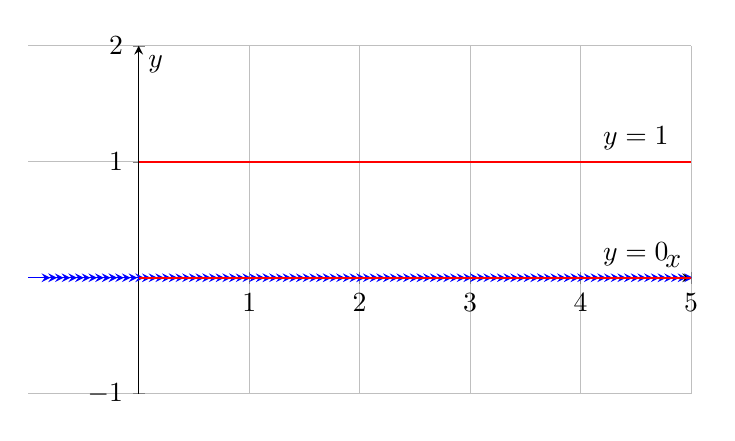
\begin{tikzpicture}
    \begin{axis}[
        axis lines = middle,
        xlabel = \(x\),
        ylabel = \(y\),
        ymin = -1, ymax = 2,
        xmin = -1, xmax = 5,
        xtick = {0,1,2,3,4,5},
        ytick = {-1,0,1,2},
        grid = both,
        width=10cm,
        height=6cm,
        domain=-1:5,
        samples=100
    ]
    % Direction field
    \addplot[blue, quiver={u=1, v={y*(1-y)}, scale arrows=0.2}, -stealth] {0};
    
    % Equilibria
    \addplot[red, thick] coordinates {(0,0) (5,0)};
    \addplot[red, thick] coordinates {(0,1) (5,1)};
    
    % Labels for equilibria
    \node at (axis cs:4.5,0.2) {\(y=0\)};
    \node at (axis cs:4.5,1.2) {\(y=1\)};
    
    \end{axis}  
  \end{tikzpicture}
  \caption{Direction field and equilibria for \(\frac{dy}{dx} = y(1-y)\).}
  \label{fig:direction-field}
\end{figure}


The direction field in Figure \ref{fig:direction-field} illustrates the behavior of solutions near the equilibria \(y=0\) and \(y=1\)..

\begin{figure}
  \centering
  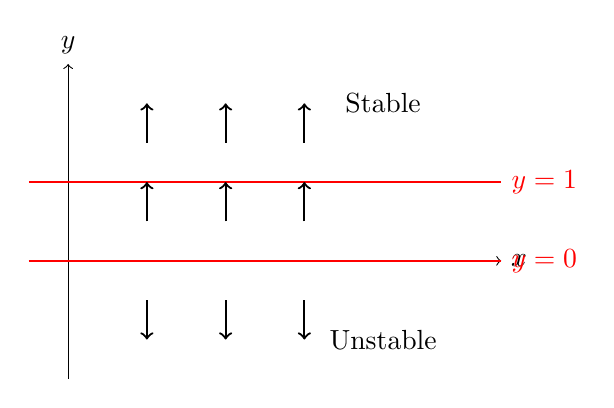
\begin{tikzpicture}
    \draw[->] (-0.5,0) -- (5.5,0) node[right] {\(x\)};
    \draw[->] (0,-1.5) -- (0,2.5) node[above] {\(y\)};
    
    % Equilibria lines
    \draw[red, thick] (-0.5,0) -- (5.5,0) node[right] {\(y=0\)};
    \draw[red, thick] (-0.5,1) -- (5.5,1) node[right] {\(y=1\)};
    
    % Arrows indicating stability
    \draw[->, thick] (1,-0.5) -- (1,-1);
    \draw[->, thick] (2,-0.5) -- (2,-1);
    \draw[->, thick] (3,-0.5) -- (3,-1);
    
    \draw[->, thick] (1,0.5) -- (1,1);
    \draw[->, thick] (2,0.5) -- (2,1);
    \draw[->, thick] (3,0.5) -- (3,1);
    
    \draw[->, thick] (1,1.5) -- (1,2);
    \draw[->, thick] (2,1.5) -- (2,2);
    \draw[->, thick] (3,1.5) -- (3,2);
    
    % Labels for stability
    \node at (4,-1) {Unstable};
    \node at (4,2) {Stable};
  \end{tikzpicture}
  \caption{Phase portrait for \(\frac{dy}{dx} = y(1-y)\).}
  \label{fig:phase-portrait}
\end{figure}
The phase portrait in Figure \ref{fig:phase-portrait} shows  the stability of the equilibria.
It is given in the diagram by arrows indicating the direction of movement of solutions near the equilibria.

\textbf{Note:} The stability of an equilibrium can often be determined by examining the sign of \(f(y)\) near the equilibrium.
If \(f(y)\) changes from positive to negative as \(y\) increases through \(y_0\), then \(y_0\) is stable.
If \(f(y)\) changes from negative to positive, then \(y_0\) is unstable.




\section{A Numerical Method for \ode{}s}
\subsection{Euler's Method}
Euler's method is a simple numerical technique for approximating the solution of an initial value problem (IVP) of the form:
\[\frac{dy}{dx} = f(x,y), \quad y(x_0) = y_0.
\]
The idea is to use the slope of the solution at a known point to estimate the value of the solution at a nearby point.
The method proceeds as follows:
\begin{enumerate}
    \item Choose a step size \(h\).
    \item Compute the next point using the formula:
    \item \[y_{n+1} = y_n + h f(x_n, y_n), \quad x_{n+1} = x_n + h.\]
    \item Repeat the process to compute subsequent points.
\end{enumerate}


\begin{example}
  Solve the IVP:
  \[\frac{dy}{dx} = y - x^2 + 1, \quad y(0) = 0.5\]
  \begin{enumerate}
    \item Using Euler's method with step size \(h = 0.2\) to approximate \(y(1)\).
    \item Using an analytical method to find the exact solution and compare it with the approximation.
  \end{enumerate}
\end{example}



\subsection*{Summary}
\begin{itemize}
    \item First-order ODEs appear in many forms; solution methods depend on type.
    \item Existence \& uniqueness depend on continuity conditions.
    \item Separable $\Rightarrow$ integrate directly.
    \item Linear $\Rightarrow$ integrating factor.
    \item Exact $\Rightarrow$ potential function.
    \item Substitution methods (homogeneous, Bernoulli) transform to solvable forms.
    \item Autonomous ODEs model time-evolving systems.
    \item Equilibria are found by setting \(f(y) = 0\).
    \item Stability determined by sign of \(f(y)\) near equilibria.
    \item Phase portraits visualize system behavior.
    \item Euler's method approximates solutions numerically.
\end{itemize}





\section{Practice for Test --- First-Order \ode{}s}

You can use the following step-by-step calculator to help you study: \url{https://goo.gl/sZEyvL}. Do not rely on it too much, though, as you will not have such help in an exam.

There is no homework due in this discussion. Instead, study from the previous weeks and additionally work through problems below.

\subsection*{Practice Problems}

\begin{question}
  For each equation below,
  \begin{compactitem}
    \item Determine whether the given \ode{} is exact, linear, or separable by identifying the functions that demonstrate the type: \(M,N\) for exact, standard form for linear, \(F,G\) for separable and perform the appropriate tests (if needed).
    \item Find the general solution of equations using the appropriate technique.
  \end{compactitem}
  \begin{enumerate}[(a)]
    \item \((4x-8y^3)y'(x) + (5x+4y) = 0\)
    \item \(y' - e^{3x + 2y} = 0\)
    \item \((x-y^3+y^2\sin(x))y'(x) - 3xy^2-2y\cos(x) = 0\)
  \end{enumerate}
\end{question}

\begin{question}
  Find the value of $k$ such that the given \ode{} is exact:\\
    \[
    y^3 + kxy^4-2x + (3xy^2+20x^2y^3)y'(x)=0
    \]
\end{question}


\begin{question}
Conceptual questions and definitions:
  \begin{compactenum}[(a)]
    \item What is the equilibrium of an \ode{}?
    \item What is the difference between general and particular solutions of an \ode{}?
    \item What determines the angle of line segments used to plot direction fields?
    \item What is an equilibrium of an \ode{}?
    \item Define what it means for an equilibrium to be stable? Then explain how one can determine if an equilibrium is stable without finding a solution of an \ode{}.
  \end{compactenum}
\end{question}


\begin{question}
  Find the fixed points, determine their stability, and sketch the phase portrait around them.
  \begin{colenumerate}
    \item \(\dot x - (x-2)(x+2)^{2}(x-7)\)
    \item \(\dot x = \cos(x) \)
    \item \(\dot x = \cos(x) + 1\)
    \item \(\dot x = \left( \frac{1}{5} - \frac{1}{x} \right)\left( \frac{1}{5} - \frac{2}{x} \right)^{2} \), for \(x > 0\)
  \end{colenumerate}
\end{question}


\begin{question}
  Use phase portrait information to determine what the solution does as \(x \to \infty\) if \(y(0) = 3\) for the \ode{}:\\
    \[
      y'(x) + (y-2)(y-4)^{2}.
    \]
\end{question}


\begin{question}
Each of these \ode{}s could be linear, separable, or exact. Identify the type of each equation and support your answer by:
  \begin{compactitem}
  \item putting the linear equation into its standard form and circling the input term,
  \item performing the exactness test on the exact equation,
    \item identifying the separated \(F\) and \(G\) components for the separable \ode{}.
    \end{compactitem}

      \begin{colenumerate}
      \item \((4y + 2t - 5) + (6y + 4t - 1)\dot y = 0\)
      \item \(x y'(x) + (3x+1)y - e^{-3x} = 0\)
    \item \(\dot N + N - N t e^{t+2} = 0\)
    \item \(\sqrt{1-y^{2}} - y'(x)\sqrt{1-x^{2}} = 0\)
    \item \( (2xy + x^{2} - 1)y'(x) + (x+y)^{2}= 0\)
    \item \( (x+2)^2 y' - 5 + 8y + 4xy = 0\)
    \item \(\sin(3x) + 2 [ \cos(3x) ]^{2} y' \cdot y = 0\)
    \item \((e^{x} + y) + (2+x+ye^{y})y'(x) = 0\).
    \item \( y' + \tan(x) y - \cos^{2}(x) = 0\)
    \end{colenumerate}
\end{question}


\begin{question}
(Challenge) Give an example of a first-order \ode{} that is neither linear, separable, or exact. Perform the tests as in the previous question that demonstrate this.
\end{question}

\begin{question}
 Find the \textbf{general solution} of each of the following equations using any technique that you find appropriate. Then, find the \textbf{particular solution} that satisfies the given initial condition.
  \begin{enumerate}[(a)]
    \item \(x^{2} y'(x) - y + xy\), \(y(-1) = -1\)
    \item \(x y'(x) + y - 4x - 1\), \(y(1) = 8\)
    \item \( (x-y^3+y^2\sin(x)) - (3xy^{2} + 2y\cos(x))y'(x) = 0 \), \(y(0) = 2\)
  \end{enumerate}
\end{question}

\begin{question}
The following equation is not exact (it fails the exactness test). Nevertheless, apply the technique for solving exact equations. At which point does the technique break down?
  \[
    (x^{2} + 2xy -y^{2}) dx + (y^{2} + 2xy - x^{2})dy = 0
  \]
\end{question}



%%% Local Variables:
%%% mode: latex
%%% TeX-master: "main"
%%% End:








